\documentclass[12pt, letterpaper]{article}
\usepackage[margin=0.85in]{geometry}
\usepackage{amsmath,amssymb,enumitem,scrextend}
\usepackage[hidelinks]{hyperref}
\usepackage{xcolor, graphicx}
\usepackage{subcaption}
\setlength{\parindent}{0in}

\begin{document}
	\title{\vspace{-1in}Real Time Neural Network System Modeling for Adaptive Control	} 
	\author{Thomas Kost}
	\date{\today}
	\maketitle
	\tableofcontents
	
	\section{Abstract}
		Non-linear systems are notoriously difficult to characterize, leaving our models of poorly-linearizable systems woefully incomplete\cite{Narendra2}. Through employing the use of a dynamic neural network (DNN) to identify out plant, we can both identify unknown aspects of our model as well as employ dynamic state feedback to control our system. We can derive a learning law for our neural networks that guarantee the error between our network's estimation of our system and the true plant vanish\cite{Christ}. This breaks the black box uncertainty\cite{Narendra} that neural networks are typically accompanied with and provides a method by which actual robust implementations using neural networks for control can be implemented. We will describe the incorporation of a DNN as a non-linear extension of the subspace method and illustrate how both persistence of excitation and Lyapanov analysis provide guarantees for the stability and convergence of the identification and control stage. We will highlight how model deficiency can be accounted for in a well posed control affine system\cite{Koko}.	
		
	\section{Introduction}
		At the time Christodoulou's paper\cite{Christ} was published, the technique of placing a neural network in parallel with plant and internal to the control loop (Figure \ref{fig:block_diagram}) was popularized but no formal guarantees had been created--making any implementation of the technique inherently risky. 

		
		\begin{figure}
		\centering
		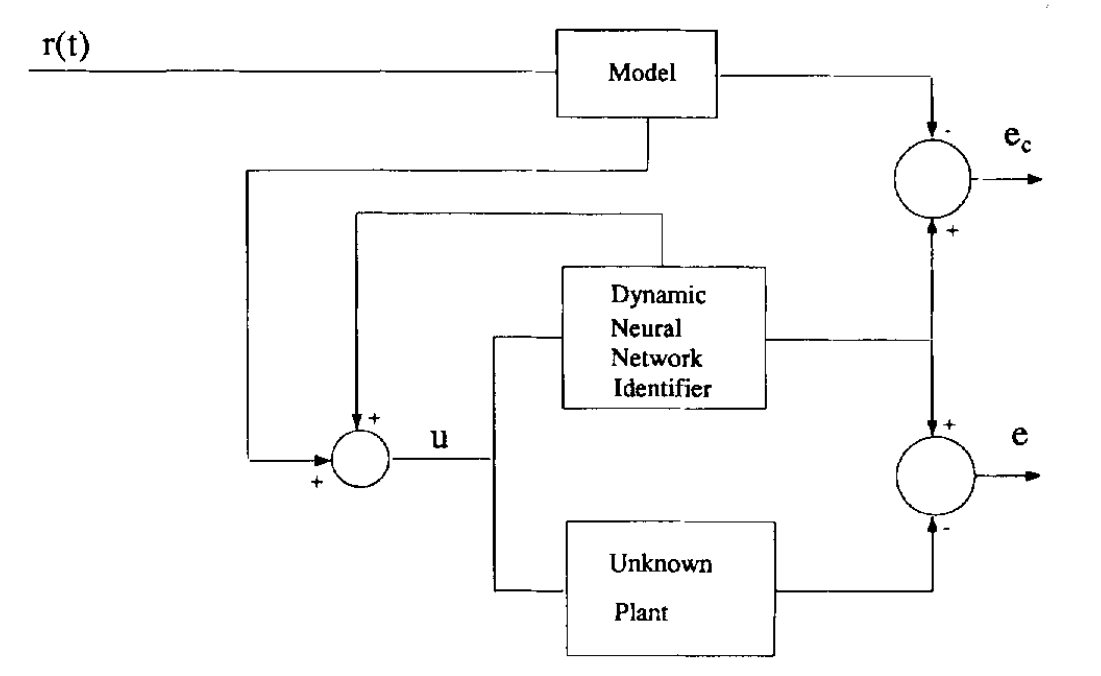
\includegraphics[width=7cm]{block_diagram.png}
		\caption{Block diagram for use of dynamic neural net}
		\label{fig:block_diagram}
		\end{figure}	
	
		Christodolou and Rovithakis applied classical Adaptive control theory (Lyapanov analysis and Barbalat's Lemma)  to provide robust guarantees on performance in terms of parametric uncertainty. This can be seen as a nonlinear extension to the classical parametric uncertainty problem for Adaptive control. Further guarantees are made for handling a rank deficient model as well--this argument is made via Single Perturbation Analysis. These guarantees form the justification of a two stage algorithm presented in the paper. The first step is the identification phase, where it is shown the DNN can approximate and (given persistence of excitation) converge to the ground truth parameters. The second step is the addition of control, where it is shown a given model reference can be tracked despite rank and parametric deficiencies when compared to the true system.
			
		In this project, we will give the relevant background for understanding Christodolou's Argument. We will then present his argument and findings--discussing applications as well. Finally, we will connect the use of a neural network to  identify and control our system to the problems of adaptive control as presents in class as well as the problem of identification (via the Subspace method\cite{Verhaegen2013}). Finally, we will discuss potential areas of future development needed in the light of Christodolou's result.
			
	\section{Stability Analysis of Dynamical Neural Networks for Adaptive Control}
	
	In this section we will walk through the argument presented for parametric and model uncertainty. For parametric uncertainty, we can characterize stability of the neural network architecture through a simple Lyapanov argument. We will need to introduce Single Perturbation Analysis, as a method for understanding these systems. As stated in the paper our system is given by:
	\begin{align}
		\dot{x} &= Ax +BW^{*}S(x)+BW^{8*}_{n+1}S'(x)u 
		\label{system}
	\end{align}
	Where $S(x)$ and $S'(x)$ are each a sigmoid function (where $S'(x) >0 $). Here, $x \in \mathbb{R}^{n}$ and all matrices are square. Note $W^{*}$ is the true value of our parameters, we will be largely working with $W$, our estimate of the parameters, and $\tilde{W} = W-W^{*}$, our error in parameters. The same notation applies to $W_{n+1}$. Additionally, $\hat{x}$ is our estimate of the state in our dynamic neural net.
	\subsection{Parametric Uncertainty(Lyapanov Stability)}
		Christodolou establishes the stability of our dynamic neural network architecture for identification and control with respect to parametric uncertainty. He does this with a straightforward Lyapanov argument. He rewrites the system in terms of the error:
		\begin{align*}
			e&= \hat{x}-x \\
			\implies \dot{e} &= Ae+B\tilde{W}S(x)+B\tilde{W_{n+1}}S'(x)u
		\end{align*}
	
		From this formulation, a simple Lyapanov function is posed (where P satisfies the Lyapanov equation):
		
		\begin{align*}
		V(e, \tilde{W}, \tilde{W_{n+1}}) &= \frac{1}{2}e^{T}Pe+\frac{1}{2}tr(\tilde{W}^{T}\tilde{W})) +\frac{1}{2}tr(\tilde{W_{n+1}}^{T}\tilde{W_{n+1}})
		\end{align*}
		Through performing some algebraic manipulation, taking the gradient along the flow, and plugging in the definition $\dot{e}$ we find:
		\begin{align*}
			\dot{V} &= \frac{1}{2}e^{T}e +S^{T}(x)\tilde{W}^{T}BPe +u^TS'(x)\tilde{W}_{n+1}^{T}BPe+tr(\dot{\tilde{W}}^{T}\tilde{W})) +tr(\dot{\tilde{W_{n+1}}}^{T}\tilde{W_{n+1}})
		\end{align*}
	We have a degree of freedom in $\dot{\tilde{W_{n+1}}}$ and $\dot{\tilde{W}}$ since we have not specified a learning rule. Christodolou suggests we judiciously choose:
	\begin{align*}
		tr(\dot{\tilde{W}}^{T}\tilde{W}) &= -S^{T}(x)\tilde{W}^{T}BPe \\
		tr(\dot{\tilde{W}}_{n+1}^{T}\tilde{W}_{n+1}) &= -u^TS'(x)\tilde{W}_{n+1}^{T}BPe\\
		\implies \dot{V} &= -\frac{1}{2}e^{T}e \leq 0
	\end{align*}
	Since $\dot{V}$ is negative semi-definite through the application of LaSalle's Invariance principle we can consider the set of $\{e, \tilde{W},\& \tilde{W_{n+1}}| \dot{V}=0\}$. Since this is the trivial trajectory, we can consider the system asymptotically stable with bounded $V$. Through integrating $V$ over all time and applying Barbalat's theorem we can show that the above learning laws will force $\lim{e(t)} \to 0$.
	
	This is easily extended to the case of control with defining:
	\begin{align*}
		e_{c} &= \hat{x}-x_{model} \\
		u &= (BW_{n+1}S'(x))^{-1}(Ax_{m}+BWS(x)-A_{m}x_{m}-B_{m}r)
	\end{align*}
	It should be noted here that additional requirements of boundedness must be met on a term by term basis for the case of control--but, but the proof remains fundamentally the same. The largest difference is a piece-wise modification to the definition of $\dot{W}$ and $\dot{W_{n+1}}$ that adds an additional negative definite term to ensure the existence of $(BW_{n+1}S'(x))^{-1}$.
	
	This gives us guarantee on the identification of our model when parameters are uncertain. There exists a concrete and implementable learning law in which we can force both our identifier states and model states to converge to the true system state. This guarantee showcases the DNN architecture as a method of creating controllers on classically difficult nonlinear systems. Christodolou further notes, convergence to the true parameters requires persistent excitation--this is commented on later in this project. 
	
	\subsection{Single Perturbation Analysis Background}
	We can also consider the situation in which our model itself is inaccurate. In identification, the assumption is often that we know the appropriate number of states to describe our system--however, we may often be privy only to a low rank understanding of our non-linear systems we with to identify and control. In order to analyze these systems we can turn to Single Perturbation Analysis (SPA)\cite{Koko}. 
	
	To perform SPA we will be considering systems of the form\cite{Koko}:
	
	\begin{align*}
	\dot{x} &= f(x,z,\epsilon,t), \; x(t_{0}) = x_{0}, \; x \in \mathbb{R}^{n} \\
	\epsilon\dot{z} &= g(x,z,\epsilon,t), \; z(t_{0}) = z_{0}, \; z \in \mathbb{R}^{m}
	\end{align*}
	
	Where $x$ describes our known (ore even measurable) states and $z$ describes our unknown dynamics. $\epsilon > 0$ is a parameter used to denote the fact that our unknown dynamics have small contribution to the overall system in that they change slowly and thus to not rapidly affect our model state. A Singular Perturbation is defined to be the change from $\epsilon >0$ to $\epsilon = 0$. This change is the perturbation required to move from our low rank model approximation to a full rank ground truth model. If we can show that given this change, our system remains asymptotically stable, then our system is robust to model errors (Dynamic Uncertainty). In other words, we can use this perturbation to characterize the magnitude of uncertainty our model can handle while still remaining stable. This is useful in estimation the region of attraction for our system--also giving us guidance as to the set of spaces for which we can guarantee stability.
	\subsection{Model Uncertainty}
	We begin with the introduction of our error states $z$. As described above, our model can be written in the following form:
	\begin{align*}
			\dot{x} &= Ax +BW^{*}S(x)+BW^{8*}_{n+1}S'(x)u + F(x,W,W_{n+1})A_{0}^{-1}B_{0}W_{0}u+F(x,W,W_{n+1})z \\
			\mu\dot{z} &= A_{0}z+B_{0}W_{0}u
	\end{align*}
	Here  $ F(x,W,W_{n+1})A_{0}^{-1}B_{0}W_{0}$ and $F(x,W,W_{n+1})z$ can be viewed as correction terms. They account for disparity between our modeling of the unknown states and the true behavior. We should also  note that our states in $z$ are written in a linear model--this is supported by the fact that we have these nonlinear general correction terms present. 
	As before we can rewrite our system in terms of the error between our estimated state and the true state. 
	\begin{align*}
			e&= \hat{x}-x \\
		\implies \dot{e} &= Ae+B\tilde{W}S(x)+B\tilde{W_{n+1}}S'(x)u -F(x,W,W_{n+1})A_{0}^{-1}B_{0}W_{0}u-F(x,W,W_{n+1})z \\
		\mu\dot{z} &= A_{0}z+B_{0}W_{0}u
	\end{align*}
	Here we must assume that the unmodeled dynamics $z$ are asymptotically stable. We should note that this is a reasonable assumption, otherwise there would be no hope for control--as our state could explode and change wildly differently from our model (making our single perturbation modeling useless). This is equivalent to all eigenvalues of $A_{0}$ having negative real part.
	
	Under these assumptions we can make a single perturbation required to change our model from $\mu >0$ to $\mu =0$. This means our unmodeled dynamics must satisfy the following condition:
	\begin{align*}
		z&= -A_{0}^{-1}B_{0}W_{0}u
	\end{align*}
	We shall now take another page from Single Perturbation Theory, we will express $z$ in terms of its fast-decaying transients, $\eta$ and its "quasi-steady state", $h(x,\eta)$. Here the quasi steady state refers to the subset of true state variables ($z$) being in steady state\cite{Koko}. Since our dynamics for $z$ after our perturbation describe a steady state we have:
	\begin{align*}
		z &= h(x,\eta) +\eta \\
		\implies h(x,\eta) &= -A_{0}^{-1}B_{0}W_{0}u
	\end{align*}
	Using this decomposition we can rewrite our system in terms of our transient and quasi-steady state:
	\begin{align*}
		\dot{e} &= Ae+B\tilde{W}S(x)+B\tilde{W}_{n+1}S'(x)u -F(x,W,W_{n+1})\eta \\
		\mu\dot{\eta} &= A_{0}\eta-\mu\dot{h}(e,\tilde{W}, \tilde{W}_{n+1}, \eta,u)
	\end{align*}
	Our aim now is to find satisfactory bounds such that we can create a valid Lyapanov function. We can describe the time derivative of $h(\cdot)$ in terms of the partial derivatives with respect to each of it's arguments and the time derivatives of each argument (total law of derivatives). Christodolou then notes that through bounding each of these derivatives we can create an upper bound:
	\begin{align*}
		||\dot{h}(e,\tilde{W}, \tilde{W}_{n+1}, \eta,u)|| &\leq \rho_{1}||e||+\rho_{2}||\eta||
	\end{align*}
	
	Given the above results and formulations, Christodolou begins another fairly straightforward Lyapanov argument to show that the error, $e$ converges to 0. He poses the following Lyapanov function:
	
	\begin{align*}
		V &= \frac{1}{2}c_{1}e^{T}Pe +\frac{1}{2}c_{2}\eta^{T}P_{0}\eta +\frac{1}{2}c_{1}tr(\tilde{W}^{T}\tilde{W})	+\frac{1}{2}c_{2}tr(\tilde{W}_{n+1}^{T}\tilde{W}_{n+1})\\
		&c_{1},c_{2} \in \mathbb{R}
	\end{align*}
	As before $P$ and $P_{0}$ satisfy the Lyapanov equation with $A$ and $A_{0}$ respectively. We now apply the learning law derived in the previous argument and assuming the upper bound on $\dot{h}(\cdot)$ to find an upper bound on $\dot{V}$\\
	TODO:
	- generation of an upper bound \\
	- formulate Vdot as quadratic\\
	- Asymptotic stability and barbalets thm to show error disappear\\
	- show the obvious extension to control as before\\
	
	- implication that we are able to use reduced order models and the architecture will self correct for errors in our modeling as it continually learns
	
	\section{Connections to Course}
	\subsection{Parametric Uncertainty in a Nonlinear System}
	In class we discussed the question of controlling a linear system with uncertain parameters. \\
	
	- Nussbaums fundamental limit on adaptive control 
	
	 
	
	\subsection{Persistence of Excitation}
	A consistent theme throughout the paper is the need for persistence of excitation for model parameters to converge within the Neural network. This is reflective of the connection to Classical Adaptive control. As in classical adaptive control, we can derive a simple regulator that will achieve stability through a monotonically increasing gain, but this makes no guarantee that our model converges to an approximation of System \ref{system}. We should recall Nussbaum's Theorem and contribution to this issue, convergence of such a system with unknown parameters required a persistence of excitation. Persistence of excitation provides continual exploration for the system, allowing for it to continually learn and update the parameters to be estimated. Similarly, Christodolou comments that this is a necessary condition for convergence of our Neural Network model. In order for the model to arrive at the true parameters, it must explore the state space adequately to form an adequate estimate. This is important for the sake of practicality in these controllers. If we want to ensure we are not simply overpowering the dynamics of the system, achieving control via a brute force, then we must form an adequate estimate of our system. Unfortunately, this condition in the nonlinear case cannot be distilled to a condition on the input alone. Since the sigmoid functions in the dynamic neural network are nonlinear functions on our state, we are unable to guarantee this explores the space adequately enough to converge\cite{Christ}.
	
	\subsection{Identification Via Projection}
	Neural Networks can be fundamentally describes as a nonlinear change of basis. In the development of neural networks for the purpose of identifying and characterizing dynamics, it is important that the network if forced to learn in a manner which uncovers the underlying dynamics\cite{Brunton}. This is often done through the choice of architecture and loss function design--however, Christodolou's paper attacks this problem through a different angle (and narrower scope). He instead finds the necessary conditions for stability of our system, and discovers the learning rate that enforces stability. As a result, the Dynamic neural net in Figure \ref{fig:block_diagram} will learn a nonlinear mapping that forces our state estimations and true states to converge (similarly with reference inputs). The Neural network in other words, projects the given model and inputs onto the true model of the system--giving the closest approximation possible allowing stability to be preserved and the identification process to converge.
	
	We can view this as an online non-linear extension to the subspace method. Rather than collecting our data all at once, we are itteritvely collecting our data and updating our estimate of the model. Similar to the subspace method, we expect poor estimations of the system when few data points have been recorded, but once we have enough data the estimate begins to converges to our best approximation of the system. We should note here that the subspace method performs a projection of our future outputs along our future inputs onto our past inputs and outputs. This is done via a pseudo-inverse as we are working in an LTI framework. However, we can note that our neural network is performing the analog task in a nonlinear framework. We note that we determine the error from our previous estimate of state and the observed value. This error is used in our update to modify our current system estimate to best predict our current state.
	\[ADD \; EQ\]
	 This learning law takes our past inputs and outputs in the form of an error signal, and modifies the current model with the present state value to give us the best estimate of future states(i.e. our error asymptotically converges to 0). 
		
	We can note too that both methods require a persistence of excitations for the true model to be completely recovered. While the neural net can create adequate performance, the parameters will only converge to the true parameters of the system when persistence of excitation is satisfied \cite{Christ}.
	
	
	
	
	\section{Shortcomings}
	While this paper provides several advancements and theoretical guarantees of DNN's, there are a few outstanding issues that are not well addressed for robust implementation in practice. One such issue is the use of the error correction term $F(x,W,W_{n+1})$. While the implicit assumption is that due to the nature of our SPA the mismatch between our neural net states and ground truth states is small, this is not garunteed. As we are working with nonlinear systems, we cannot guarantee that small perturbations will not result in larger disparities in the state. Since for stability we ask that $F(x,W,W_{n+1})$ be bounded, our argument becomes the unknown mismatch must be small for the mismatch to disappear. While the logic is sound, it loses impact in application where model uncertainty of a nonlinear system is difficult to bound. Furthermore, we run into the all too common issue with nonlinear systems, where the system itself may have wide ranging behavior, in which such a restriction further reduces the ball of states which we can operate on safely.
	
	Another shortcoming is in the actual substance of the result. All Lyapanov functions and control schemes are designed such that they are negative semi-definite. For a nonlinear system this implies only asymptotic stability, which has no guarantees as to the rate of convergence of our identification nor our control law. The stronger result of exponential stability requires showing Input to State Stability and a Lyapanov function of the form $\dot{V} \leq -\lambda V$. Showing this case would give a guarantee as to the rate of decay for our Lyapanov function. Without this, we cannot reasonably guarantee that the identification phase of our DNN will converge to an acceptable approximation of the system in a reasonable amount of time. While this is something the engineer can design around empirically, no theoretical guarantees are made. It should be noted that this is no fault of the author--finding Lyapanov functions is a difficult task in and of itself. Finding Control Lyapanov Functions (CLFs) of the form mentioned above are even more challenging. For systems where feedback linearization and backstepping cannot be easily applied (the same systems in which we intend to use a DNN)--it becomes a much taller order. 
	


	\section{Future Development}

	Potential future extensions would be the determination of Safety and barrier functions for these systems. If we can provide formal guarantees of the safety of neural networks we can further adopt these systems without concern of them damaging hardware or sensitive equipment. 
	
	TODO: further reading in the field
	\bibliographystyle{plain}
	\bibliography{bib}
		\nocite{*}
\end{document}